% Source: fixed 2006 Zhejiang science scan, PDF page 1, Q15.
% The plotted phase is schematic but respects the transcribed closed range
% 0 <= phi <= pi/2; M and N are adjacent x-intercepts around peak P.
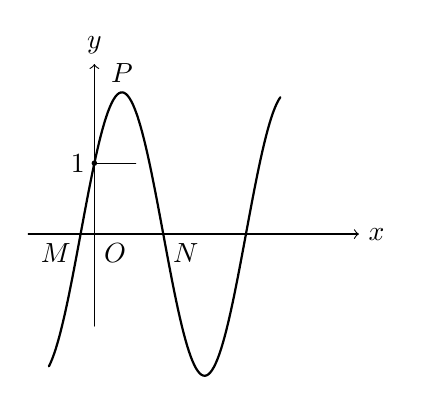
\begin{tikzpicture}[line cap=round,line join=round,x=1.05cm,y=0.9cm]
  \draw[->] (-0.8,0)--(3.2,0) node[right] {$x$};
  \draw[->] (0,-1.3)--(0,2.4) node[above] {$y$};
  \draw[thick] plot[domain=-0.55:2.25,samples=130] (\x,{2*sin(180*\x+30)});
  \draw (0,1)--(0.5,1);
  \node[left] at (0,1) {$1$};
  \fill (0,1) circle (1pt);
  \node[above] at (1/3,2) {$P$};
  \node[below left] at (-1/6,0) {$M$};
  \node[below right] at (5/6,0) {$N$};
  \node[below right] at (0,0) {$O$};
\end{tikzpicture}
